\section{Middleware}

As we already mentioned, the Worldwide LHC Computing Grid is a
distributed computing infrastructure that spans over five continents
managing resources distributed across the world (due to  funding,
operability and access reasons). The resources operated by the WLCG
belong either to the two main global grids, EGI \cite{EGI} and OSG \cite{OSG}, or
to other collaborating regional or national grids. To make this
diverse variety of resources globally available for all the WLCG
users, the WLCG has been developing its own middleware, a software
layer that ``brings all the resources together'': a collection of
programs, services and protocols to manage and operate the entire
WLCG infrastructure (see Figure~\ref{fig09}).

%fig09
\begin{figure}[htb] % h-here, t-top, b-bottom
\centering
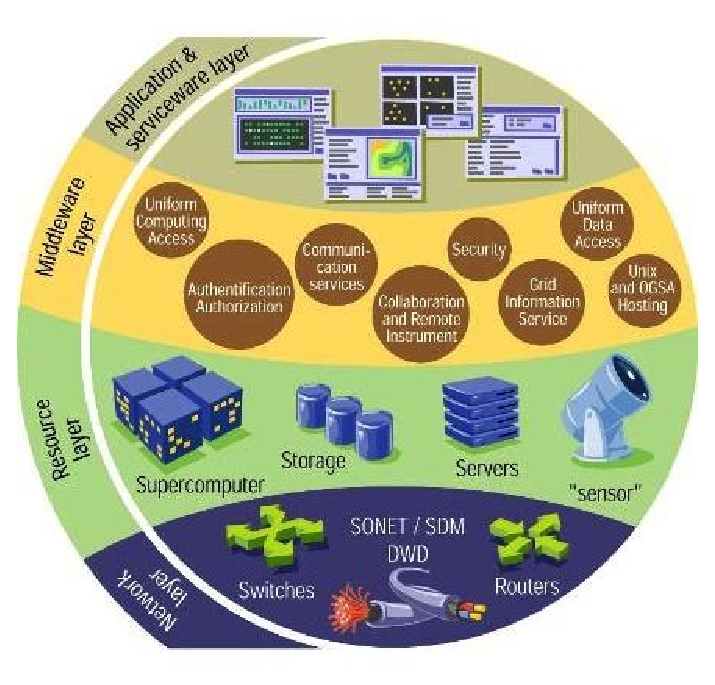
\includegraphics[width=13cm]{fig09.eps} %    ** if .eps don't need extension
\caption{Grid Layers}\label{fig09}
\end{figure}



\subsection{Overview of Grid services}
%
The WLCG middleware is a complex suite of packages which includes
(see also Figure~\ref{fig10}):

\begin{itemize}
\item Data Management Services:
%
\begin{itemize}
\item Storage Element
\item File Catalogue Service
\item Grid file access tools
\item File Transfer Service
\item GridFTP service
\item Database and DB Replication Services
\item POOL Object Persistency Service
\end{itemize}
%
\item Security Services:
%
\begin{itemize}
\item Certificate Management Service
\item Virtual Organization \cite{VO} Management Registration Service (VOMRS)
\item Authentication and Authorization Service (the X509 infrastructure)
\end{itemize}
%
\item Job Management Services:
%
\begin{itemize}
\item Compute Element
\item Workload Management
\item Service VO Agent Service
\item Application Software Install Service
\end{itemize}
%
\item Information Services:
%
\begin{itemize}
\item Accounting Service
\item Site Availability Monitor
\item Monitoring tools: experiment dashboards; site monitoring
\end{itemize}
%
\end{itemize}

%fig10
\begin{figure}[htb] % h-here, t-top, b-bottom
\centering
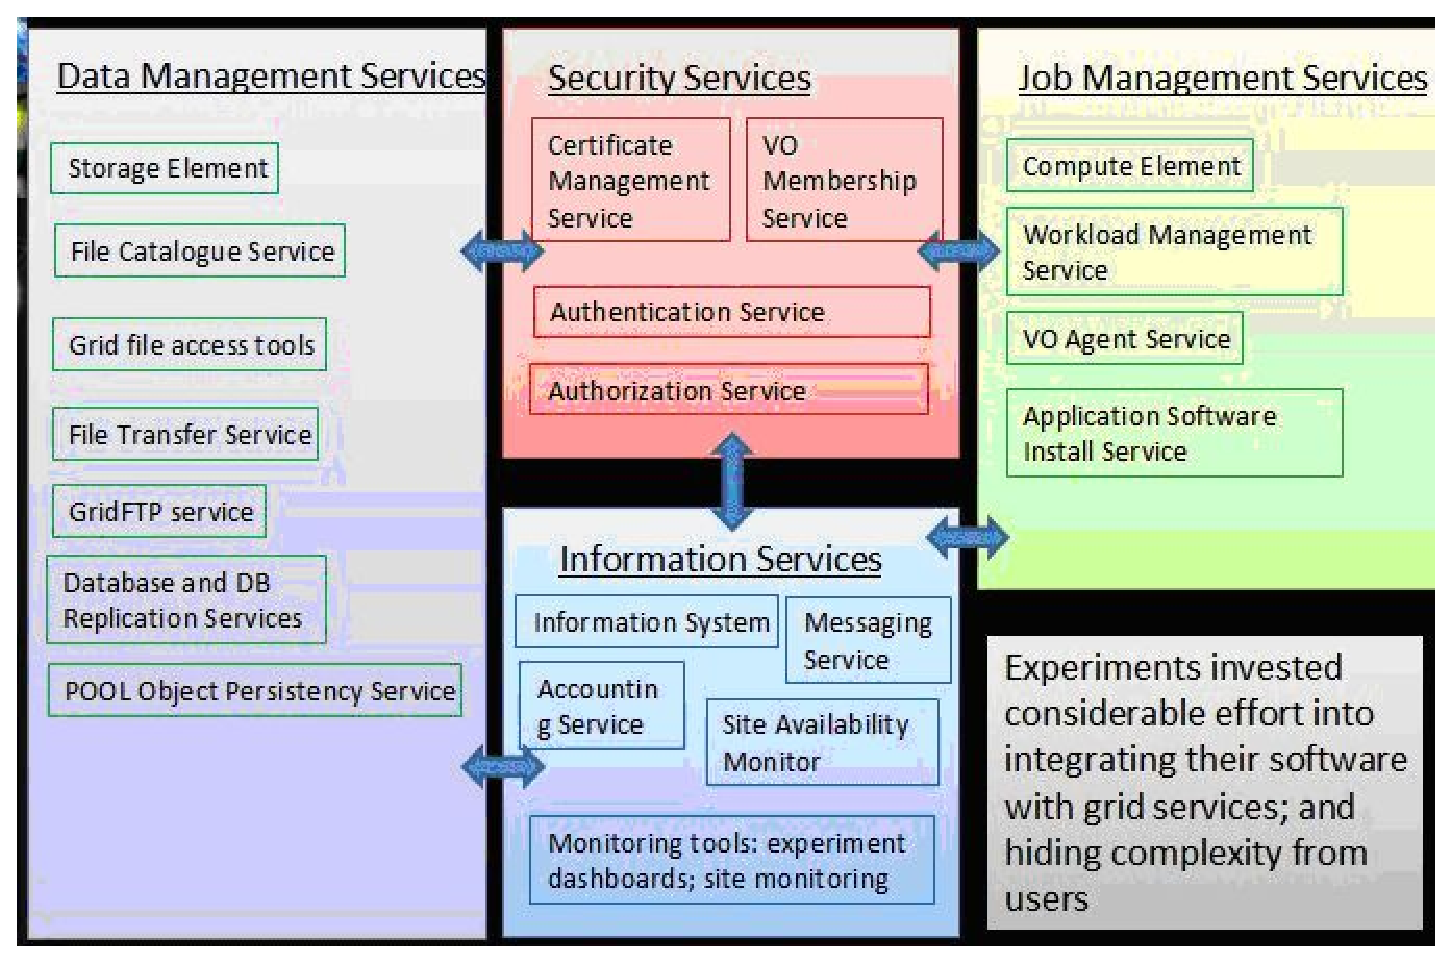
\includegraphics[width=13cm]{fig10.eps} %    ** if .eps don't need extension
\caption{Schema of Grid services}\label{fig10}
\end{figure}



The WLCG middleware has been built and further developed using and
developing some packages produced by other projects including, e.g.:
%
\begin{itemize}
\item EMI (European Middleware Initiative)\cite{EMI}, combining the key
middleware providers of ARC, gLite, UNICORE and dCache
\item Globus Toolkit \cite{globus} developed by the Globus Alliance
\item OMII from the Open Middleware Infrastructure Institute \cite{OMII}
\item Virtual Data Toolkit \cite{VDT}
\end{itemize}

\subsection{Experiments' specific developments}
%
All the LHC experiments created their own specific Computing models
summarized in the individual Computing Technical Design Reports (TDRs).
They do not rely only on the WLCG-provided middleware packages
but are also developing
some specific components tailored to better comply with their
Computing models.

For example, the ALICE experiment has developed a grid middleware
suite AliEn  (AliCE Environment \cite{AliEn}), which provides a single
interface for a transparent access to computing resources for the
ALICE community. AliEn consists of a collection of components and
services which will be described in the next section. AliEn, together
with selected packages of the WLCG-provided middleware, gives a
complete framework to the ALICE community to manage and process the
data produced by the LHC according to the ALICE Computing model.

All the LHC experiments invested a considerable effort into
shielding the users from the underlying complexity of the Grid
machinery, trying to provide relatively simple entry points into the
Grid. This effort has payed off and is reflected in a considerable
number of physicists actually using the WLCG for their analysis.

\subsection{Selected WLCG-provided services}
%
In the following section, we will describe as an example the
Computing model of the ALICE experiment. The WLCG services used in
this model include the Computing Element (CE), the Storage Element
(SE) and the VOBOX.

\subsubsection{Computing Element}
%
The Computing Element (CE) \cite{CE} is a middleware component/grid
service providing an entry point to a grid site. It authenticates
users and submits jobs to Worker Nodes (WN), aggregates and
publishes information from the nodes. It includes a generic
interface to the local cluster called Grid Gate (GG), Local Resource
Management System (LRMS) and the collection of Worker Nodes.

Originally, the submission of jobs to CEs was performed by the Workload
Management System (WMS) \cite{WMS}, a middleware component/grid service,
that also monitors jobs status and retrieves their output. WLCG
(gLite) CE is a computing resource access service using standard
grid protocols. To improve the performance, the CREAM (Computing
Resource Execution And Management) Computing Element \cite{CREAMCE} has
replaced the gLite-CE in production since 2009. It is a
simple, lightweight service for job management operation at the
Computing Element level. CREAM-CE accepts job submission requests
(described with the same files as used for the Workload Management
System) and other job management requests like e.g. job monitoring.
CREAM-CE can be used by a generic client, e.g. an end-user willing
to directly submit jobs to a CREAM-CE, without the WMS component.

\subsubsection{Storage Element (XRootD)}
%
The Storage Element (SE) \cite{SE} provides storage place and access for
data. Important variables apart from available storage space,
read/write speeds and bandwidth concern reliability against
overload, percentage of failed transfers from/to SE and percentage
of lost/corrupted files.

WLCG (gLite) provides dCache \cite{dcache} and DPM \cite{dpm} storage management
tools used by the LHC experiments. However within the ALICE
infrastructure, the preferred storage manager is the Scalla/XRootD
package \cite{xrootd} developed within a SLAC \cite{slac} - CERN collaboration
(originally, it was a common project of SLAC and INFN \cite{INFN}). After
CERN got involved, the XRootD was bundled in ROOT \cite{ROOT} as a generic
platform for distributed data access, very well suited for the LHC
data analysis.

The primary goal has been the creation of data repositories with no
reasonable size limit, with high data access performance and linear
scaling capabilities. The framework is a fully generic suite for
fast, low latency and scalable data access, which can serve any kind
of data, organized as a hierarchical filesystem-like namespace,
based on the concept of directory.

``xrootd'' is just the name of the data access daemon. Although
fundamental, it is just a part of the whole suite. The complete
suite is called Scalla/XRootD, Scalla meaning Structured Cluster
Architecture for Low Latency Access.

The manager exhibits important features including:
%
\begin{itemize}
\item High speed access to experimental data
\item High transaction rate with rapid request dispersement (fast
open, low latency)
\item Write once read many times processing mode
\item Fault tolerance (if servers go, the clients do not die)
\item Fault tolerance (able to manage in realtime distributed
replicas)
\item Integrated in ROOT
\end{itemize}

From the site administrator point, the following features are
important:
\begin{itemize}
\item  No database requirements (no backup/recovery issues, high
performance)
\item Resources gentle, high efficiency data server (low
CPU/byte overhead, small memory footprint)
\item  Simple installation
\item Configuration requirements scale linearly with site complexity
\item No 3rd party software needed (avoids messy dependencies)
\item Low administration costs
\item Self-organizing servers remove need for
configuration changes in big clusters
\end{itemize}

Additional features:
\begin{itemize}
\item Generic Mass Storage System Interface (HPSS, CASTOR, etc)
\item Full POSIX access
\item Server clustering for scalability, supports large number of
clients from a small number of servers
\item Up to 262000 servers per cluster
\item High WAN data access efficiency (exploit the throughput of
modern WANs for direct data access, and for copying files as well)
\end{itemize}

\subsubsection{VOBOX}
%
The VOBOX \cite{VOBOX} is a standard WLCG service developed in 2006 in order
to provide the LHC experiments with a place where they can run their
own specific agents and services. In addition, it
provides the file system access to the experiment software area.
This area is share between VOBOX and the Worker Nodes at the given
site.  In the case of ALICE, the VOBOX is installed at the WLCG sites on dedicated machines
and its installation is mandatory for sites to enter the grid
production (it is an "entry door" for a site to the WLCG
environment). The access to the VOBOX is restricted to the Software
Group Manager (SGM) of the given Virtual Organization. Since 2008,
this WLCG service has been VOMS-aware [34]. In the following
section, we will describe the services running on the VOBOX machines
reserved at a site for the ALICE computing.
